
\chapter{提案手法}
\label{cpt:提案手法}

\section{提案手法}
\section{定義}

\begin{dfn}[許容重みなしBanach空間$X$]
  \label{dfn:Banach-l1}
  Banach空間$X$を次のように定める.はじめに$l^1$空間を次のように定める.
  \begin{equation}
    l^1 := \left\{ a=(a_k)_{k\in \mathbb{Z}} : a_k \in \mathbb{C}, \|a\| := \sum_{k \in \mathbb{Z}} |a_k| < \infty \right\}
  \end{equation}
  そして,検証に用いる関数空間$X$は
  \begin{equation}
    X:= \mathbb{C} \times l^1, x = (\omega, a), \omega \in \mathbb{C}, a \in l^1
  \end{equation}
  と定め,そのノルムを
  \begin{equation}
    \| x \|_X := \max \{ |\omega| , \|a\| \}
  \end{equation}
  として定義する.このとき,$X$はBanach空間となる.
\end{dfn}

\begin{dfn}[拡張したヤコビ行列$DF(x)$]
  \label{dfn:拡張したヤコビ行列}
  まず,近似解$x$について
  \begin{equation}
    x = (\omega,\ \underbrace{0,\cdots,0}_{M},\ a,\ \underbrace{0,\cdots,0}_{M}) \in \mathbb{C}^{2N+2M}
  \end{equation}
  と定めると,$F(x)$のヤコビ行列は
  \begin{equation}
    DF(x) = \left[
      \begin{array}{c|ccc}
        0 & \cdots & 1 & \cdots \\ \hline
        \vdots & & \vdots &  \\
        \partial_w f_k & \cdots & \partial_{a_j}f_k & \cdots \\
        \vdots & & \vdots &
      \end{array}
    \right] %\in \mathbb{C}^{(2N+2M) \times (2N+2M)}
  \end{equation}
  と定義できる.
\end{dfn}

\begin{dfn}[作用素$A_M$の定義]
  \label{dfn:作用素A}
  はじめに,
  \begin{equation}
    \bar{x} = (\omega,\ \underbrace{0,\cdots,0}_{M},\ a,\ \underbrace{0,\cdots,0}_{M}) \in \mathbb{C}^{2N+2M}
  \end{equation}
  と定めると,$A_M$の定義は,以下のように定義できる.
  \begin{equation*}
    A_M = \left(
    \begin{array}{c|ccc}
      DF(\bar{x})^{-1} & 0 & \cdots & \cdots \\ \hline
      0 & \lambda_N^{-1} &  & 0 \\
      \vdots &  & \lambda_{N+1}^{-1} &  \\
      \vdots & 0 &   & \ddots
    \end{array}
    \right)
  \end{equation*}
\end{dfn}

\section{計算手順}

$A=DF(\bar{x})^{-1}$とおき,$\| AF(\bar{x}) \| \leq Y_0$に代入すると,節\ref{sct:無限次元ガウスの消去法}より,
\begin{equation}
  \left \| DF(\bar{x})^{-1} F(\bar{x}) \right \| \leq Y_0
\end{equation}
となる.ここで,
\begin{equation*}
  \phi:=DF(\bar{x})^{-1} F(\bar{x})
\end{equation*}
とおくと,
\begin{equation*}
  DF(\bar{x}) \phi = F(\bar{x})
\end{equation*}
と変形できる.$\Pi_N$を射影演算子とすると,
\begin{equation}
    \begin{split}
    \begin{pmatrix}
      \Pi_N DF(\bar{x}) \Pi_N & \Pi_N DF(\bar{x}) (I-\Pi_N) \\
      (I-\Pi_N) DF(\bar{x}) \Pi_N & (I-\Pi_N) DF(\bar{x}) (I-\Pi_N)
    \end{pmatrix}
    \begin{pmatrix}
      \Pi_N \phi \\
      (I-\Pi_N) \phi
    \end{pmatrix}
    \\=
    \begin{pmatrix}
      \Pi_N F(\bar{x}) \\
      (I - \Pi_N) F(\bar{x})
    \end{pmatrix}
  \end{split}
\end{equation}
となり,両辺に$A_M$を掛けて
\begin{equation}
  \label{eq:y0-1}
  \begin{split}
  A_M
    \begin{pmatrix}
      \Pi_N DF(\bar{x}) \Pi_N & \Pi_N DF(\bar{x}) (I-\Pi_N) \\
      (I-\Pi_N) DF(\bar{x}) \Pi_N & (I-\Pi_N) DF(\bar{x}) (I-\Pi_N)
    \end{pmatrix}
    \begin{pmatrix}
      \Pi_N \phi \\
      (I-\Pi_N) \phi
    \end{pmatrix}
    \\=A_M
    \begin{pmatrix}
      \Pi_N F(\bar{x}) \\
      (I - \Pi_N) F(\bar{x})
    \end{pmatrix}
  \end{split}
\end{equation}
となる.ここで,線形作用素$T,B,C,E$それぞれに対し,
\begin{equation*}
  \begin{split}
    T:= \Pi_N ADF(\bar{x}) \mid _{X_1}:X_1 \rightarrow X_1,\quad &
    B:= \Pi_N ADF(\bar{x}) \mid _{X_2}:X_2 \rightarrow X_1, \\
    C:= (I-\Pi_N) ADF(\bar{x}) \mid _{X_1}:X_1 \rightarrow X_2,\quad &
    E:= (I-\Pi_N) ADF(\bar{x}) \mid _{X_2}:X_2 \rightarrow X_2
    \label{eq:def_lo}
  \end{split}
\end{equation*}
と定義でき,式(\ref{eq:y0-1})を次のように変形できる.
\begin{equation}
  \begin{pmatrix}
    T & B \\
    C & E
  \end{pmatrix}
  \begin{pmatrix}
    \Pi_N \phi \\
    (I -\Pi_N) \phi
  \end{pmatrix}
  =
  \begin{pmatrix}
    \Pi_N A F(\bar{x}) \\
    (I - \Pi_N) A F(\bar{x})
  \end{pmatrix}
\end{equation}

線形作用素$S$を,
定理\ref{thm:6.2.1-L全単射}より,線形作用素$S$を
\begin{equation*}
  S:=E-CT^{-1}B:X_2 \rightarrow X_2
\end{equation*}
とする.もし,$S$が全単射ならば,
\begin{equation*}
  \begin{pmatrix}
    \Pi_N \phi \\
    (I-\Pi_N)\phi
  \end{pmatrix}
  =
  \begin{pmatrix}
    T^{-1}+T^{-1}BST^{-1} & -T^{-1}BS^{-1} \\
    -S^{-1}CT^{-1} & S^{-1}
  \end{pmatrix}
  \begin{pmatrix}
    Pg \\
    (I-P)g
  \end{pmatrix}
\end{equation*}
となり,有界線形作用素$ADF(\bar{x})$は全単射となる.

$S$について計算する.式(\ref{eq:def_lo})より,
\begin{equation}
  \begin{split}
    S &= E-CT^{-1}B \\
    &= \left( \left( I-\Pi_N \right) ADF ( \bar{x} ) \right) - (\left( I-\Pi_N \right) ADF( \bar{x} )) (\Pi_N ADF(\bar{x}))^{-1} ((I-\Pi_N)ADF(\bar{x}))
  \end{split}
  \label{eq:s-def}
\end{equation}
となる.ここで,
\begin{equation*}
  \| I_{X_2} -S \| < 1
\end{equation*}
であれば,$S$は全単射となる.




\chapter{実験結果}
\section{実験環境}
本研究を行った実験環境を表\ref{tab:環境},使用したパッケージを表\ref{tab:パッケージ}を示す.

\begin{table}[h]
  \centering
  \caption{実験環境}
  \label{tab:環境}
  \begin{tabular}{c||c}
    環境 & 詳細 \\ \hline
    CPU & 12th Gen Intel(R) CORE(TM) i7-12700 \\
    OS & Linux(x86_64-linyc-gnu)\\
    Julia & Version 1.11.2
  \end{tabular}
\end{table}

\begin{table}[h]
  \centering
  \caption{使用パッケージ}
  \label{tab:パッケージ}
  \begin{tabular}{c||l}
    パッケージ & バージョン \\  \hline
    DifferentialEquations & v7.10.0 \\
    FFMPEG & v0.4.1 \\
    FFTW & v1.7.1 \\
    ForwardDiff & v0.10.36 \\
    GenericFFT & v0.1.6 \\
    IntervalArithmetic & v0.20.9 \\
    Plots & v1.39.0
  \end{tabular}
\end{table}

\section{実験結果}
実験結果の数値を表\ref{tab:norm-num}に,グラフにしたものを図\ref{fig:norm-gra}に示す.

\begin{table}[htbp]
  \centering
  \caption{フーリエサイズとノルム値}
  \label{tab:norm-num}
  \begin{tabular}{c||c}
    フーリエサイズ & $\| I_{X_2}-S \|$ \\ \hline
    50 & 0.22815114629236252 \\
    100&0.11455533660051737\\
    150&0.07655718822651922\\
    200&0.05749210273025131
\end{tabular}
\end{table}

\begin{figure}[htbp]
  \centering
  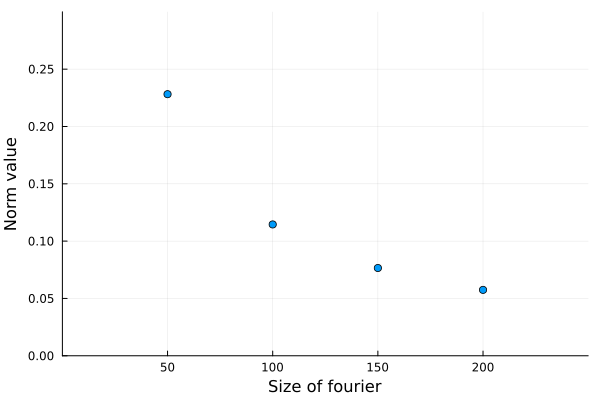
\includegraphics[scale=0.5]{img/scatter.png}
  \caption{フーリエサイズとノルム値のグラフ}
  \label{fig:norm-gra}
\end{figure}
